\section{The optical downlink}
\label{sec:outline}
\graphicspath{{_Intro/Figures/}}

\subsection{Common terminology}
\label{subsec:outlineTerminology}
This sub--section outlines optical terminology used in the rest of the text.
\subsubsection{Radiant flux}
\label{subsubsec:radiantFlux}
Radiant flux is the amount of radiant energy emitted per unit time by an optical source. Let $P(\lambda)$ be the SPD under consideration. The radiant flux $\Phi_{W}$ corresponding to the SPD is given by 
\begin{equation}
	\Phi_{\text{W}} = \int\limits_{\lambda_{\text{min}}}^{\lambda_{\text{max}}}P(\lambda)d\lambda
	\label{eqRadiantFlux}
\end{equation}
(Units: W).

\subsubsection{Radiant intensity}
\label{subsubsec:radiantIntensity}
Radiant intensity is the amount of radiant flux emitted per unit solid angle by an optical source. (Units: W/sr)

\subsubsection{Irradiance}
\label{subsubsec:irradiance}
Irradiance is the amount of radiant flux received by a surface/device per unit area. (Units: W/m$^{2}$)

\subsubsection{Luminous flux}
\label{subsubsec:luminousFlux}
Luminous flux is the amount of luminous energy emitted per unit time by an optical source. Let $P(\lambda)$ be the SPD under consideration. The luminous flux $\Phi_{lm}$ corresponding to the SPD is given by \cite{gru08b}
\begin{equation}
	\Phi_{\text{lm}} = 683\int\limits_{380\text{ nm}}^{780\text{ nm}}P(\lambda)V(\lambda)d\lambda
	\label{eqLuminousFlux}
\end{equation}
where $V(\lambda)$ is the eye sensitivity function. (Units: lm).

\subsubsection{Luminous intensity}
\label{subsubsec:luminousIntensity}
Luminous intensity is the amount of luminous flux emitted per unit solid angle by an optical source. (Units: lm/sr)

\subsubsection{Illuminance}
\label{subsubsec:illuminance}
Illuminance is the amount of luminous flux received by a surface/device per unit area. (Units: lm/m$^{2}$)

\subsection{The optical signal chain}
\label{subsec:outlineDownlink}

A practical OWC system operates under the hybrid wireless model paradigm using the visible light communication (VLC) channel as the high capacity downlink and another medium for the uplink. This seems to be the accepted model and a reasonable assumption \cite{rah15a}. \figurename{ \ref{fig:VLCdownBD}} illustrates a block diagram for a typical downlink using the optical spectrum.

\subsubsection{Data source}
\label{subsubsec:outlineSource}
The source is an entity that, while performing its tasks, produces or replicates information that needs to be communicated to another entity. 

\subsubsection{Coder}
\label{subsubsec:outlineCoder}
The coder assigns a binary bit sequence to the information from the source. In this process, it may introduce redundancy to reduce the effect of noise and interference in the channel. 

\subsubsection{Illumination state}
\label{subsubsec:outlineIllumination}
The illumination state sets the average output flux and the spectral power distribution (SPD) to be produced by luminaire(s). This is a result of a number of factors such as (a) requested illumination level by users in the space (b) optimal energy usage (c) output of `smart' applications such as circadian control, etc...

\begin{figure}[!t]
	\centering
		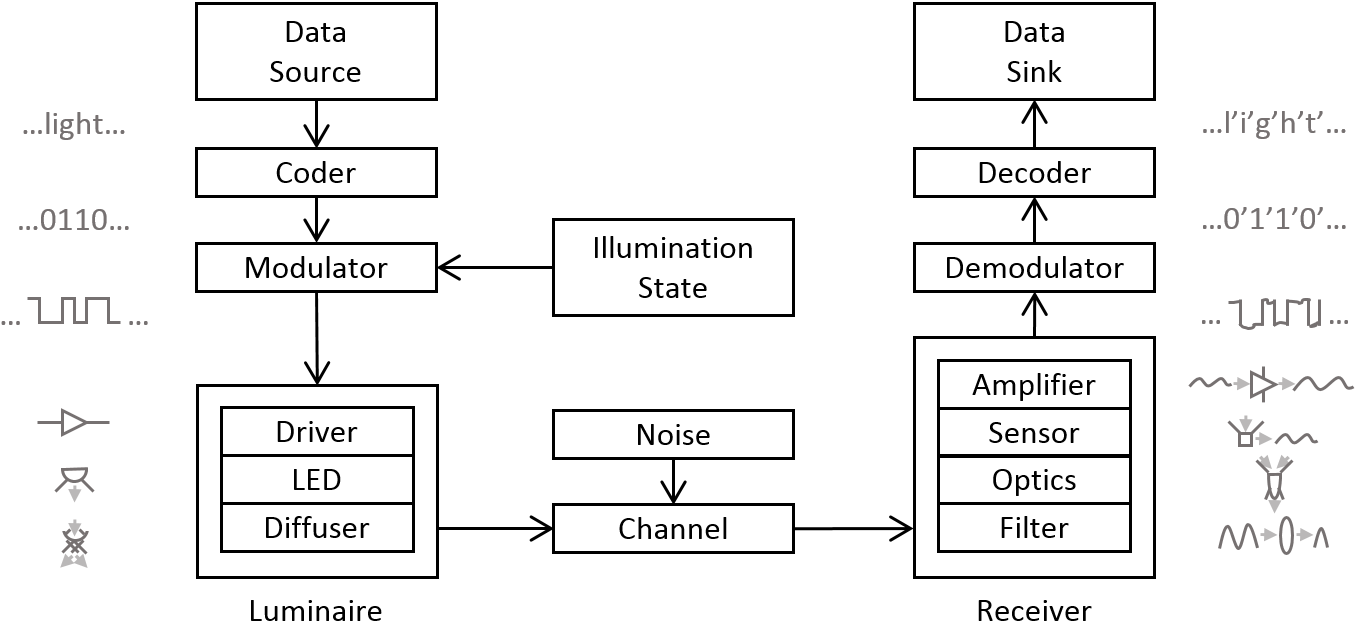
\includegraphics[width=6in]{vlcdownlinkBD.png}
	\caption{OWC downlink block diagram}
	\label{fig:VLCdownBD}
\end{figure}

\subsubsection{Modulator}
\label{subsubsec:outlineModulator}
The modulator, with the knowledge of requested flux, maps and converts the bit sequence into a corresponding waveform that drives the luminaire. The frequency of visible light is in the range of about 380 THz -- 780 THz. The current state-of-art electronics cannot sample and process signals at that high speeds. Thus traditional modulation schemes which vary the amplitude, frequency or phase of the waveforms within the RF spectrum cannot be directly implemented within the visible spectrum. Instead, the average power (a.k.a flux/intensity) of the visible waveforms are modulated to transmit data. Optical sensors like photodiodes (PD) produce output current proportional to the intensity of the incident radiation and not the waveform of the radiation itself. This signaling scheme is known as IM/DD. All optical modulation techniques are implemented in conjunction with IM/DD. This method introduces unique constraints that differentiate optical modulation techniques from RF modulation techniques.

\subsubsection{Luminaire/Transmitter}
\label{subsubsec:outlineLuminaire}
The luminaire is composed of a driver, LEDs and diffuser optics. A simple LED driver is a trans--conductance amplifier whose input is the waveform produced by the modulator. The corresponding output current drives the LED which in turn generates light. A luminaire is made up of number of phosphor converted white LEDs or different narrow--band devices which produce different colors. A phosphor converted white LED is made by coating a blue LED with yellow phosphor. The blue light excites the yellow phosphor and together they produce white light. The diffuser scatters the light produced by the LED(s) to mix the different colors and output a relatively homogenous, glare--free light which makes the luminous surface appear softer and more pleasing to the eye. Different diffuser front ends generate different sizes of cones of emission. The most common emission pattern is the Lambertian pattern. 

\subsubsection{Channel}
\label{subsubsec:outlineChannel}
The channel is the medium through which information flows. It is made up of all the paths traveled by the light rays between the luminaire and the receiver. Depending on the number of transmitters, colors or number of receiving elements, the channel can be configured into a various single/multiple input single/multiple output configurations. For the OWC downlink, the indoor space acts as the channel. In addition to the line-of-sight (LOS) path from the luminaire to the receiver, various reflected rays of light propagating over different path lengths may be incident on the receiver. In an RF system, such multi--paths cause inter-symbol-interference (ISI) that needs to be resolved for. In the indoor OWC system, due to poor reflectivity off various walls and directionality of receiving optics, optical signals propagating over such multi--paths have been shown to be heavily attenuated when incident on the active element of the receiver. In addition, difference in path lengths between LOS and non-LOS (NLOS) propagation within indoor spaces is very small. This produces a small delay spread which is insignificant when compared to frequency of intensity modulation.

\subsubsection{Receiver}
\label{subsubsec:outlineReceiver}
A receiver is made up of an optical filter, refractive optics, an optical sensor like PD and an amplifier. Some high speed systems transmit data over a small range of wavelengths (ex blue (400 nm -- 500 nm)) while the entire visible spectrum is used for illumination. In such cases, a blue filter is used to remove noise from parts of the optical spectrum that do not carry any information. For wavelength division multiplexed (WDM) systems where data is transmitted independently over different parts of the spectrum, multiple non--overlapping filters are used to decorrelate the different streams of information. For single pixel receivers, concentrator optics are used to increase the effective area of the sensor while keeping its capacitance at a minimum. A number of single pixel receivers can be configured in a matrix pattern to realize a non--imaging multiple element receiver. For imaging receivers, imaging optics are used to help decorrelate the multiple channels. Sensor devices such as p-i-n junction photodiode (PIN-PD), avalanche photodiode (APD) or complementary metal oxide semiconductor (CMOS) active pixel devices generate an electrical signal proportional to radiant flux incident on the sensor. This electrical signal is amplified and conditioned before it is processed to recover transmitted information. Randomness in photon arrival and sensing gives rise to shot noise within the system. Amplifiers such as trans--impedance amplifiers (TIA) introduce thermal noise into the system. This noise then distorts the signal waveform and can cause errors in information recovery.

\subsubsection{Demodulator}
\label{subsubsec:outlineDemodulator}
With prior knowledge of the modulation scheme implemented, the demodulator makes an intelligent estimate of the transmitted signal waveform. After recovering the transmitted waveform, it de--maps it to recover the transmitted bit sequence. Significant noise that is not orthogonal to the signal waveform can introduce errors in the demodulated sequence.

\subsubsection{Decoder}
\label{subsubsec:outlineDecoder}
The decoder, with prior knowledge of the coding scheme implemented, tries to recover the transmitted information from the bit stream. Redundancy introduced in the coded data can help the decoder to detect and rectify errors.

\subsubsection{Data sink}
\label{subsubsec:outlineSink}
Ideally, the data sink is the entity to which the information was transmitted to. 
